\documentclass[12pt]{article}

\usepackage[utf8]{inputenc}
\usepackage[T1]{fontenc}
\usepackage[catalan]{babel}
\usepackage{lmodern}
\usepackage{geometry}
\usepackage{hyperref}
\usepackage[dvipsnames]{xcolor}
\usepackage[bf,sf,small,pagestyles]{titlesec}
\usepackage{titling}
\usepackage[font={footnotesize, sf}, labelfont=bf]{caption} 
\usepackage[font={footnotesize, sf}, labelfont=bf]{subcaption}
\usepackage{siunitx}
\usepackage{graphicx}
\usepackage{booktabs}
\usepackage{amsmath,amssymb}
\usepackage[sort]{cleveref}
\usepackage{enumitem}

\geometry{
	a4paper,
	right = 2.5cm,
	left = 2.5cm,
	bottom = 3cm,
	top = 3cm
}

\hypersetup{
	colorlinks,
	linkcolor = {red!50!blue},
	linktoc = page
}

\crefname{figure}{figura}{figures}
\crefname{table}{taula}{taules}
\numberwithin{table}{section}
\numberwithin{equation}{section}
\numberwithin{figure}{section}

\graphicspath{{./figs/}}

% Unitats
\sisetup{
	inter-unit-product = \ensuremath{ \cdot },
	allow-number-unit-breaks = true,
	detect-family = true,
	list-final-separator = { i },
	list-units = single
}

\newcommand{\Z}{\mathbb{Z}}
\renewcommand{\vec}[1]{\mathbf{#1}}
\newcommand{\N}{\mathbb{N}}
\newcommand{\R}{\mathbb{R}}
\newcommand{\C}{\mathbb{C}}
\newcommand{\Ry}{\mathit{Ry}}
\let\Im\relax
\let\Re\relax
\let\div\relax
\DeclareMathOperator{\Im}{Im}
\DeclareMathOperator{\Re}{Re}
\DeclareMathOperator{\div}{div}
\newcommand{\abs}[1]{\lvert #1 \rvert}
\newcommand{\inn}[2]{\left\langle #1 , #2 \right\rangle}
\newcommand{\parbreak}{
	\begin{center}
		--- $\ast$ ---
	\end{center} 
}
\makeatletter
\newcommand*{\defeq}{\mathrel{\rlap{%
    \raisebox{0.3ex}{$\m@th\cdot$}}%
  \raisebox{-0.3ex}{$\m@th\cdot$}}%
	=
}
\makeatother

\newpagestyle{pagina}{
	\headrule
	\sethead*{\sffamily {\bfseries Seminari 2:} {\sffamily Teoremes de Poincaré-Bendixson i Bendixson-Dulac}}{}{\theauthor}
	\footrule
	\setfoot*{}{}{\sffamily \thepage}
}
\renewpagestyle{plain}{
	\footrule
	\setfoot*{}{}{\sffamily \thepage}
}
\pagestyle{pagina}

\title{\sffamily {\bfseries Seminari 2:} {\sffamily Teoremes de Poincaré-Bendixson i Bendixson-Dulac}}
\author{\sffamily Arnau Mas}
\date{\sffamily 16 de maig de 2019}

\begin{document}
\maketitle

\addtocounter{section}{1}
\section*{Problema 1}
Hem d'analitzar la dinàmica de dues poblacions regides pel sistema d'equacions 
\begin{equation} \label{eqn:dinàmica de poblacions}
	\left\{
		\begin{aligned}
			\dot{x} &= x(1 - x - ay) \\
			\dot{y} &= y(1 - y - bx)
		\end{aligned}
	\right.
\end{equation}
on \( a \) i \( b \) són paràmetres positius. En primer lloc veiem que l'origen sempre és un punt crític del sistema, així com els punts \( (0,1) \) i \( (1,0) \). També tenim que els dos eixos són invariants. D'aquesta manera ens podem restringir al primer quadrant, la qual cosa és natural si pensem que \( x \) i \( y \) modelen poblacions, de manera que ambdues han de ser positives.   

A continuació farem el retrat de fase del sistema quan almenys un dels dos paràmetres és diferent de 1. Per a fer els retrats de fase és útil considerar les nulclines del camp, és a dir, les corbes sobre les quals una de les dues components del camp és nu\l.la. És clar que els dos eixos són nulclines. D'altra banda també ho són les rectes d'equacions \( x + ay = 1 \), sobre la qual la component horitzontal del camp s'anu\l.la, i \( bx + y = 1 \), sobre la qual s'anu\l.la la component vertical. A les interseccions de dues nulclines per diferents components del camp hi apareixen punts crítics. L'origen es correspon amb la intersecció dels dos eixos, el punt \( (0,1) \) és la intersecció de l'eix vertical i la recta \( bx + y = 1 \), i el punt \( (1,0) \) és la intersecció de l'eix horitzontal amb la recta \( x + ay = 1 \). Així veiem que el sistema tindrà un quart punt crític a la intersecció de les rectes \( x + ay = 1 \) i \( bx + y = 1 \), que és el punt \( \left(\frac{1 - a}{1 - ba}, \frac{1 - b}{1 - ba}\right) \). Si \( a = 1 \) o \( b = 1 \) aquest punt passa a ser \( (0,1) \) o \( (1,0) \), respectivament. Si \( ab = 1 \) aleshores les nulclines no es tallen ja que són para\l.leles. I si \( ab > 1 \) almenys un dels paràmetres ha de ser major que 1. Si només un dels dos ho és ---és a dir, \( a < 1 < b \) o \( b < 1 < a \)---, però, el punt de tall de les nulclines passa a estar fora del primer quadrant, i per tant el deixem de considerar.  El sistema, doncs, té quatre punts crítics si \( a \) i \( b \) són ambdos majors o menors que 1, i tres si un dels paràmetres és major o igual que 1 i l'altre menor que 1 o a la inversa. 

Analitzem el caràcter dels punts fixos. La diferencial del camp és
\begin{equation} \label{eqn:diferencial}
	dX(x,y) = \begin{pmatrix}
		1 - 2x - ay & -ax \\
		-by & 1 - 2y -bx
	\end{pmatrix}.
\end{equation}
Independenment del valor dels paràmetres,
\begin{equation*}
	dX(0,0) = \begin{pmatrix}
		1 & 0 \\ 0 & 1
	\end{pmatrix}
\end{equation*}
i per tant l'origen és sempre repulsor. 

Als punts \( (1,0) \) i \( (0,1) \) hi tenim
\begin{equation*}
	dX(1,0) = \begin{pmatrix}
		-1 & -a \\
		0 & 1 - b
	\end{pmatrix} \text{ i } 
	dX(0,1) = \begin{pmatrix}
		1 - a & 0 \\
		-b & -1
	\end{pmatrix}.
\end{equation*}
Fem l'anàlisi pel punt \( (1,0) \). El determinant de la diferencial en aquest punt és \( b - 1 \), de manera que serà hiperbòlic sempre que \( b \neq 1 \). Si \( b < 1 \) aleshores el determinant és negatiu i el punt serà una sella. Si \( b > 1 \) aleshores el determinant és positiu i ens cal la traça, que és \( -b \) i per tant negativa. En aquest cas el punt és atractor.  

Pel que fa al punt \( (0,1) \), el determinant de la diferencial és \( a - 1 \) i la traça \( -a \). Així, el mateix anàlisi que hem fet abans és vàlid, és a dir, serà una sella per a \( a < 1 \) i un atractor per a \( a > 1 \). 

Finalment analitzem el quart punt crític. Aquí, la diferencial és
\begin{equation*}
	dX\left(\frac{1 - a}{1 - ba}, \frac{1 - b}{1 - ba}\right) = \frac{1}{1 - ba} \begin{pmatrix}
		a - 1 & a(a-1) \\
		b(b-1) & b -1
	\end{pmatrix}.
\end{equation*}
El determinant, per tant, és
\begin{equation*}
	\frac{(a - 1)(b-1)}{1 - ab}.
\end{equation*}
Recordem que el punt que estem considerant només existia si tant \( a \) com \( b \) eren més grans que 1 o més petits que 1, és a dir, si \( (a-1)(b-1) > 0 \). En el primer cas \( ab > 1 \) de manera que el determinant és negatiu, mentre que en el segon \( ab < 1 \) i per tant el determinant és positiu. Així podem concloure que si \( a \) i \( b \) són els dos més grans que 1 aleshores el punt serà una sella. En el cas de determinant positiu, la traça de la diferencial és
\begin{equation*}
	\frac{a + b -2}{1 - ab}.
\end{equation*}
El determinant era positiu quan \( ab < 1 \), que passava quan tant \( a \) com \( b \) eren menors que 1. Així \( a+b < 2 \) i per tant la traça és negativa i per tant el punt és atractor. 

\begin{figure}[htb]
	\centering
	\begin{subfigure}[htb]{0.48\textwidth}
		\centering
		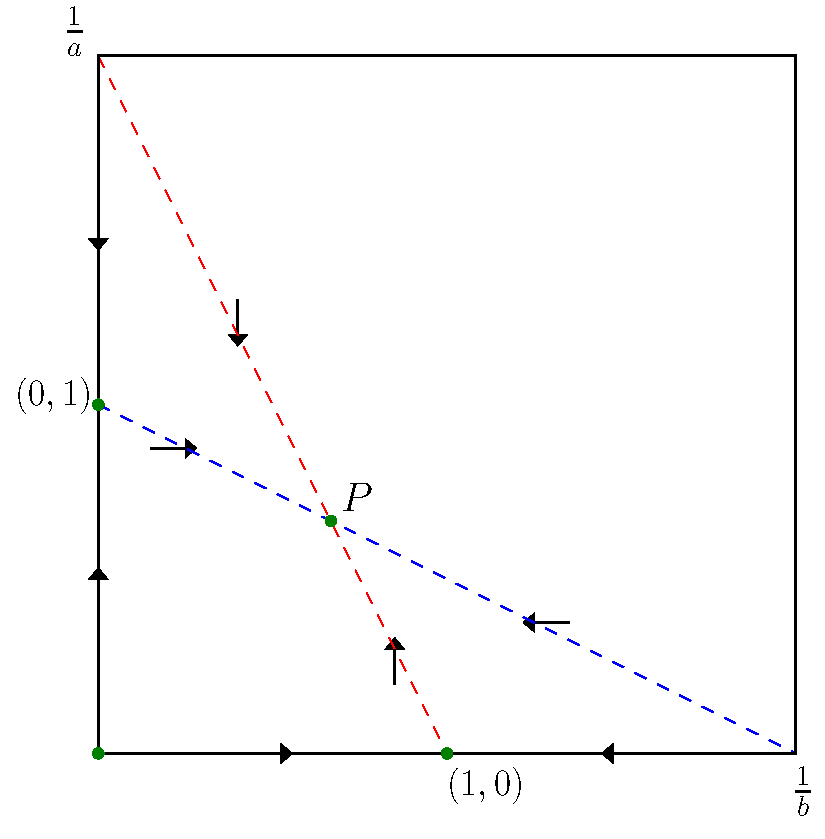
\includegraphics[width=\textwidth]{retrat-1a.pdf}
		\caption{Regions invariants del pla i nulclines}
		\label{fig:retrat 1a}
	\end{subfigure}
	\begin{subfigure}[htb]{0.48\textwidth}
		\centering
		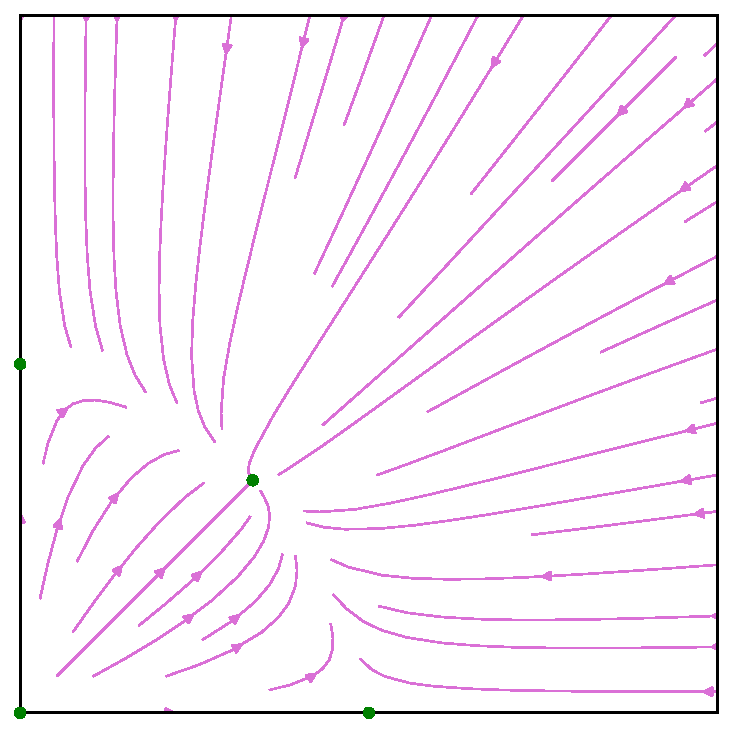
\includegraphics[width=\textwidth]{retrat-1b.pdf}
		\caption{Retrat de fase}
		\label{fig:retrat 1b}
	\end{subfigure}
	\caption{Anàlisi del sistema en el cas \( a,b < 1 \)}
\end{figure}

Un cop sabem el comportament dels punts crítics estem en condicions de determinar els retrats de fase. Considerem primer el cas \( a,b < 1 \). En aquestes condicions \( (1,0) \) i \( (0,1) \) són selles i el punt \( P = \frac{1}{1 - ba}(1 - a, 1-ba) \) un atractor.  El flux sobre els eixos és repulsor quan \( x \), \( y < 1 \) i atractor quan \( x \), \( y > 1 \). Sobre la nulclina d'equació \( ax + y = 1 \), que està representada en vermell, el flux és cap avall quan \( by + x > 1 \) i cap amunt quan \( by + x < 1 \), per tant canvia segons si estem per sota o per sobre de la nulclina d'equació	\( x + by = 1 \). I el flux sobre aquesta segueix el patró anàleg, tal i com veiem a la \cref{fig:retrat 1a}. D'aquesta manera, el pla queda dividit en quatre regions invariants. Observem que no hi pot haver cap òrbita periòdica continguda a alguna de les regions, ja que si fos així hauria d'envolatr un punt crític, i el sistema no té cap més punt crític que els 4 que hem trobat. Tampoc podria envoltar cap dels tres punts crítics sobre els eixos, ja que hauria de sortir del primer quadrant, el qual és invariant. L'única possibilitat seria una òrbita periòdica que envoltés el punt \( P \), però aleshores es veuria obligada a entrar a algun dels dos triangles positivament invariants. Sabem que \( (1,0) \) i \( (0,1) \) són selles, i la direcció d'arribada de cadascun és l'eix sobre el que es troben, per tant l'únic possible candidat a \( \omega \)-límit dins dels dos triangles invariants és \( P \) ---de fet, \( P \) és l'únic possible candidat a \( \omega \)-límit---. D'aquesta manera, quan l'òrbita periòdica entrés a algun dels dos triangles invariants es veuria obligada a morir a \( P \), la qual cosa no és possible.

Al quadrilàter delimitat pels quatre punts crítics, que és negativament invariant, (gairebé) totes les òrbites són heteroclíniques amb \( \alpha \)-límit l'origen i \( \omega \)-límit \( P \). Com que és compacta, per Poincaré-Bendixson l'únic candidat a \( \alpha \)-límit és l'origen, tret de les dues òrbites que tenen \( \alpha \)-límit a \( (0,1) \) i \( (1,0) \) ---com que són selles, hi ha una òrbita que hi neix i una que hi mor---. Totes les òrbites que neixen a l'origen o a \( (1,0) \) i \( (0,1) \) han d'atravessar les nulclines i morir a \( P \). Dins d'aquests dos triangles no hi pot néixer cap òrbita més enllà de les dues òrbites que neixen a \( (1,0) \) i \( (0,1) \), ja que no hi ha cap altre punt crític. Finalment, a la regió no fitada, ambdues components del camp són negatives i per tant totes les òrbites han d'atravessar les nulclines i morir a \( P \).

\begin{figure}
	\centering
	\begin{subfigure}[htb]{0.48\textwidth}
		\centering
		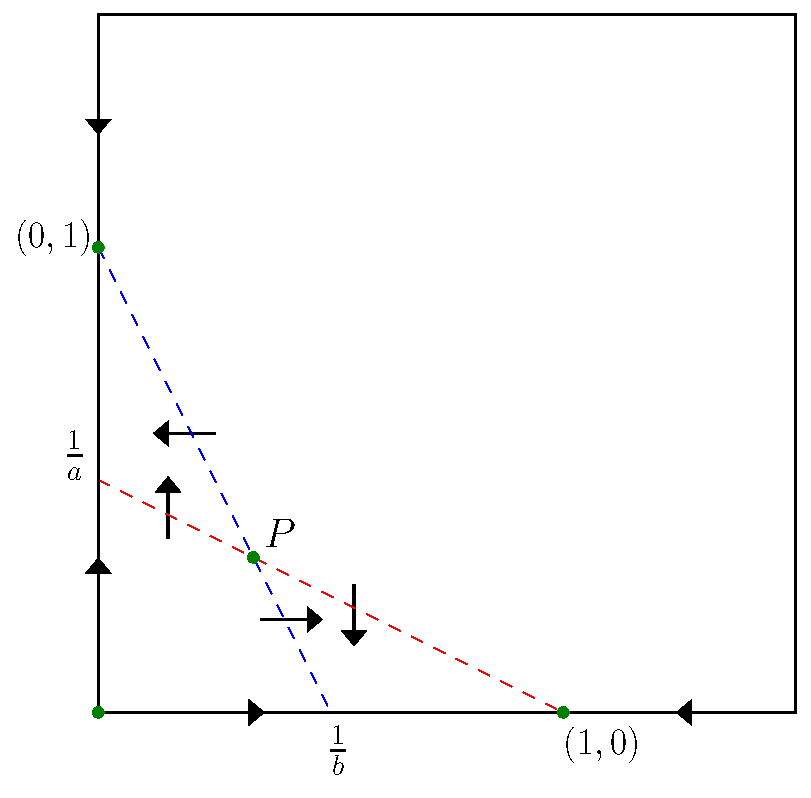
\includegraphics[width=\textwidth]{retrat-2a.pdf}
		\caption{Regions invariants del pla i nulclines}
		\label{fig:retrat 2a}
	\end{subfigure}
	\begin{subfigure}[htb]{0.48\textwidth}
		\centering
		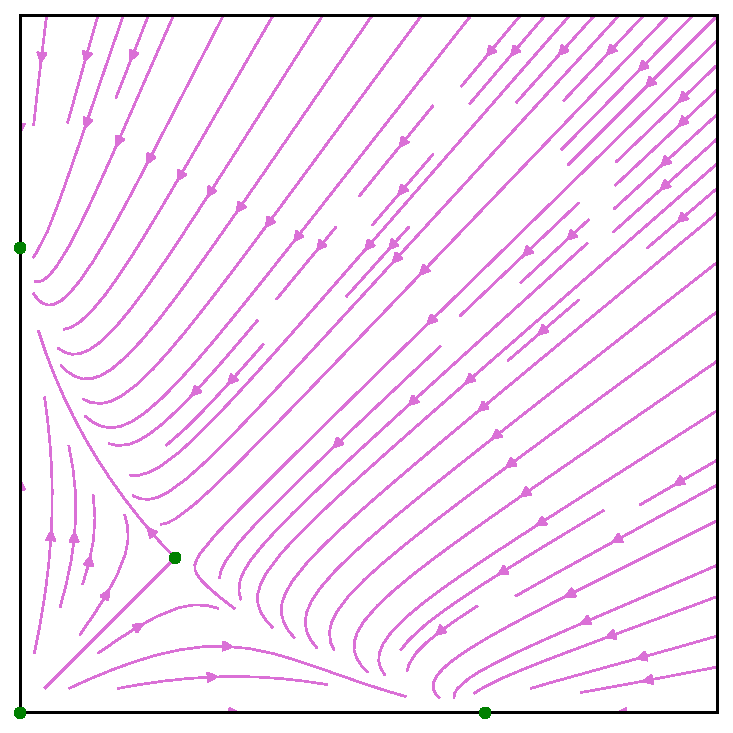
\includegraphics[width=\textwidth]{retrat-2b.pdf}
		\caption{Retrat de fase}
		\label{fig:retrat 2b}
	\end{subfigure}
	\caption{Anàlisi del sistema en el cas \( a,b > 1 \)}
	\label{fig:retrat 2}
\end{figure}

Quan \( a, b > 1 \) hem vist que \( P \) passava a ser una sella i \( (0,1) \) i \( (1,0) \) es convertien en atractors. Pel mateix argument qua abans, no poden existir òrbites periòdiques. Ara, al quadrilàter delimitat pels punts crítics les òrbites neixen totes a l'origen i han de morir a \( (0,1) \) i \( (1,0) \), tret d'una que té \( \omega \)-límit \( P \), ja que \( P \) és una sella. Aquesta òrbita és la separatriu entre les òrbites que moren a \( (0,1) \) i les que moren a \( (1,0) \). Hi ha dues òrbites que neixen a \( P \), i com que es troben dins dels triangles invariants, els seus \( \omega \)-límits han de ser \( (0,1) \) i \( (1,0) \). Finalment, el camp a la regió no fitada té els dos components negatius, per tant les òrbites en aquesta regió tenen \( \alpha \)-límit buit i \( \omega \)-límit \( (1,0) \) o \( (0,1) \), separades per l'òrbita que mor a \( P \). Tot això es pot veure a la \cref{fig:retrat 2}.

\begin{figure}
	\centering
	\begin{subfigure}[htb]{0.48\textwidth}
		\centering
		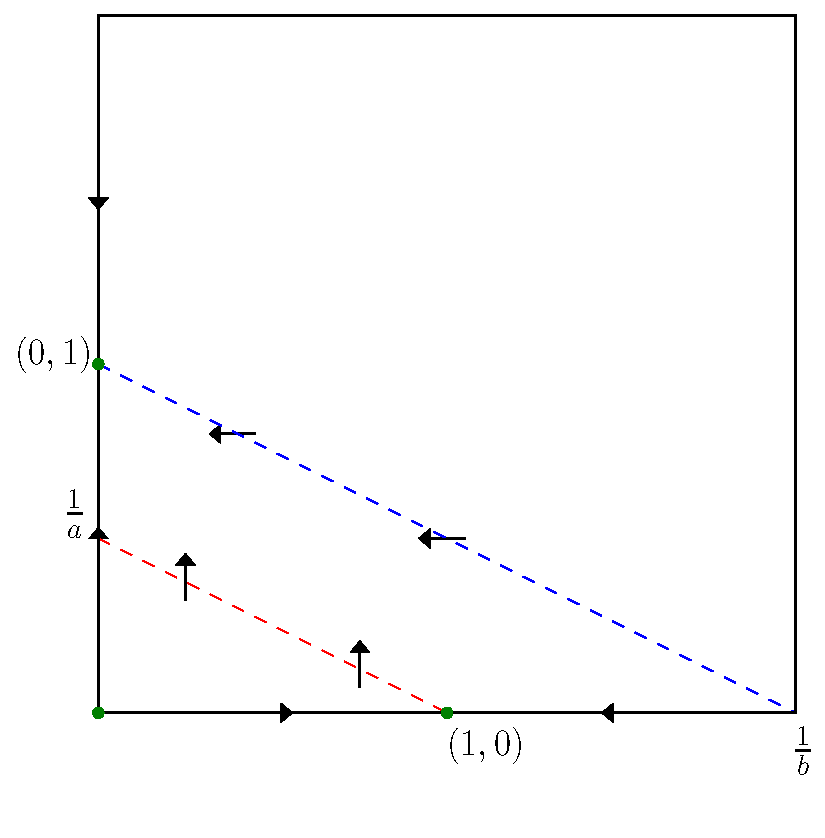
\includegraphics[width=\textwidth]{retrat-3a.pdf}
		\caption{Regions invariants del pla i nulclines}
		\label{fig:retrat 3a}
	\end{subfigure}
	\begin{subfigure}[htb]{0.48\textwidth}
		\centering
		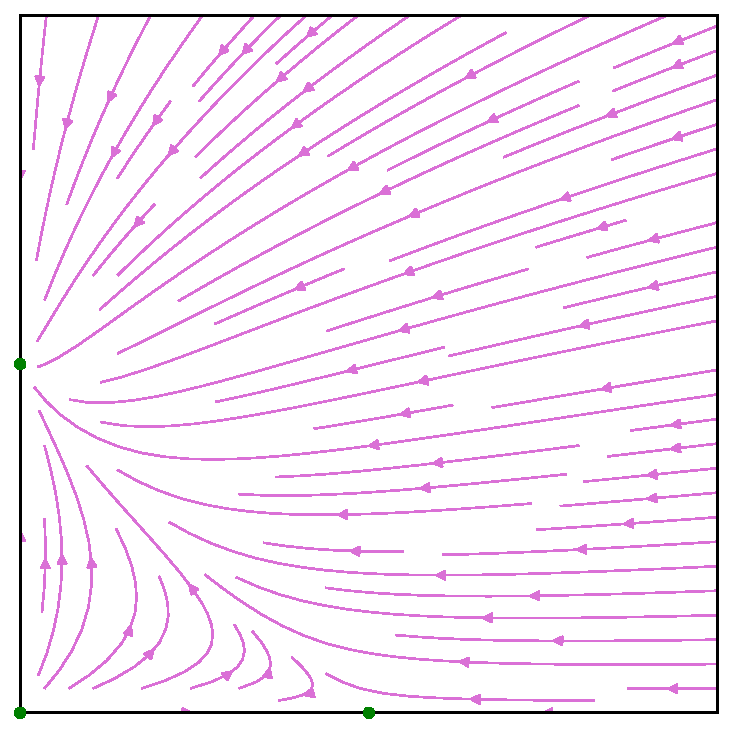
\includegraphics[width=\textwidth]{retrat-3b.pdf}
		\caption{Retrat de fase}
		\label{fig:retrat 3b}
	\end{subfigure}
	\caption{Anàlisi del sistema en el cas \( a > 1 > b \)}
	\label{fig:retrat 3}
\end{figure}
A continuació analitzem el cas \( a > 1 > b \). En aquestes circumstàncies, les nulclines ja no es tallen dins del primer quadrant i per tant tenim només tres punts fixos, dels quals \( (0,1) \) és un atractor i \( (1,0) \) una sella. Com que ara tots els punts crítics es troben sobre els eixos, no poden existir òrbites periòdiques, ja que haurien d'envoltar algun punt crític a l'interior del primer quadrant. Les nulclines separen el primer quadrant en tres regions invariants. D'una banda, el triangle delimitat per la nulclina d'equació \( x + ay = 1 \), que és negativament invariant. Totes les òrbites que neixen a l'origen han de creuar la nulclina inferior i entren a una regió positivament invariant compacta, de manera que per Poincaré-Bendixson el seu \( \omega \)-límit ha de ser \( (0,1) \). L'òrbita que neix a \( (1,0) \) també es troba dins de la mateixa regió invariant i per tant té \( \omega \)-límit \( (0,1) \). Aquesta òrbita actua com a separatriu amb les òrbites de la regió no fitada, que un cop creuen la nuclina superior es troben dins d'una regió invariant compacta, i per tant, per Poincaré-Bendixson, el seu \( \omega \)-límit també ha de ser \( (0,1) \). El corresponent retrat de fase es mostra a la \cref{fig:retrat 3}.

El cas \( b > 1 > a \) dóna lloc a un retrat de fase que és el resultat de reflectir el retrat de la \cref{fig:retrat 3} respecte la diagonal, ja que si intercanviem les components del camp ens trobem en la situació anterior. Aleshores \( (1,0) \) passaria a ser atractor i \( (0,1) \) sella.

\begin{figure}
	\centering
	\begin{subfigure}[htb]{0.48\textwidth}
		\centering
		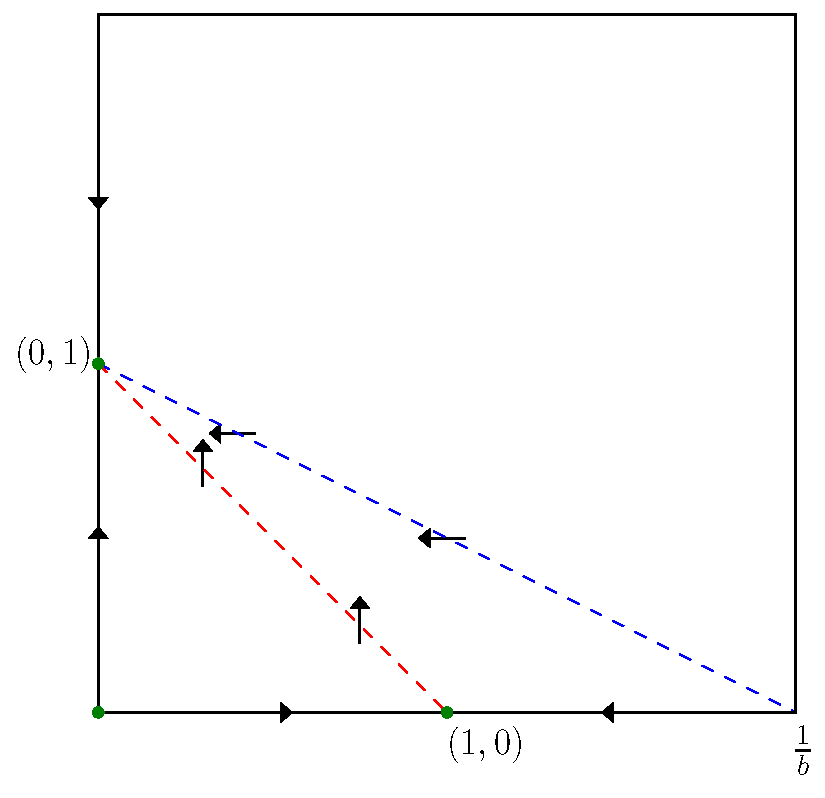
\includegraphics[width=\textwidth]{retrat-4a.pdf}
		\caption{Regions invariants del pla i nulclines}
		\label{fig:retrat 4a}
	\end{subfigure}
	\begin{subfigure}[htb]{0.48\textwidth}
		\centering
		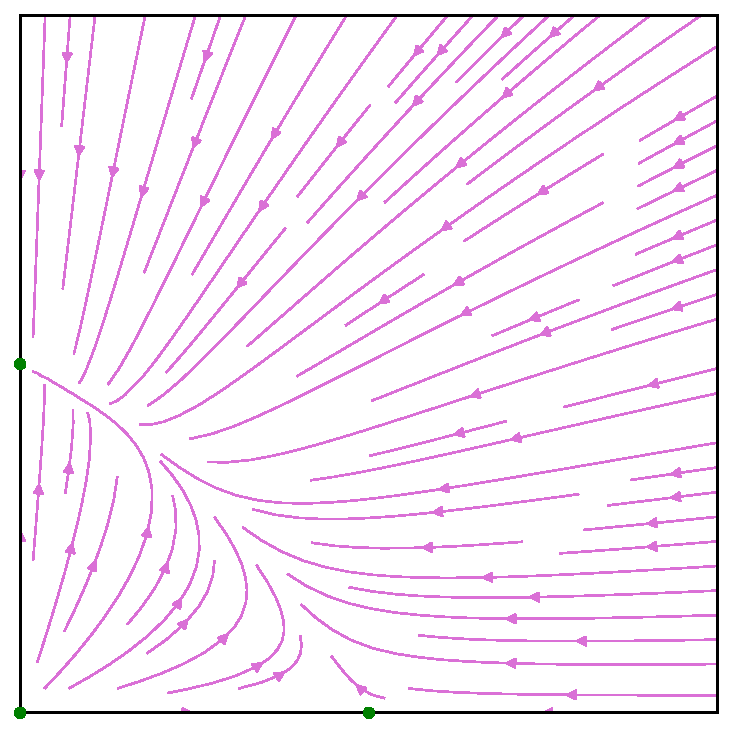
\includegraphics[width=\textwidth]{retrat-4b.pdf}
		\caption{Retrat de fase}
		\label{fig:retrat 4b}
	\end{subfigure}
	\caption{Anàlisi del sistema en el cas \( a = 1 \), \( b < 1 \)}
	\label{fig:retrat 4}
\end{figure}
Fins ara hem vist els casos on tots els punts crítics són hiperbòlics i per Hartman podem conèixer el seu comportament local abans de fer el retrat de fase. Quan \( a = 1 \) o \( b = 1 \), hi ha punts fixos que ja no són hiperbòlics, com hem vist quan hem calculat els corresponents determinants. A continuació discutim els casos amb \( a = 1 \). La situació amb \( b = 1 \), és, novament, idèntica, simplement reflectint els retrats de fase. 

Si \( a = 1 \) i \( b < 1 \) aleshores \( (1,0) \) es manté hiperbòlic i és una sella, però \( (0,1) \) deixa de ser hiperbòlic, ja que el determinant de la diferencial a \( (0,1) \) és 0 si \( a = 1 \). Aleshores no podem aplicar el teorema de Hartman. Ara bé, observem que la regió delimitada per les dues nulclines és positivament invariant i no té òrbites periòdiques, ja que envoltarien algun punt crític, de manera que tota òrbita que hi entri ha de tenir \( \omega \)-límit \( (0,1) \), ja que sabem que \( (1,0) \) és sella. I tota òrbita entra en aquesta regió, ja que les components del camp són positives per sota de la nulclina entre \( (0,1) \) i \( (1,0) \), i negatives per sobre de l'altra nulclina. Així doncs concloem que de fet \( (0,1) \) és atractor. 

\begin{figure}
	\centering
	\begin{subfigure}[htb]{0.48\textwidth}
		\centering
		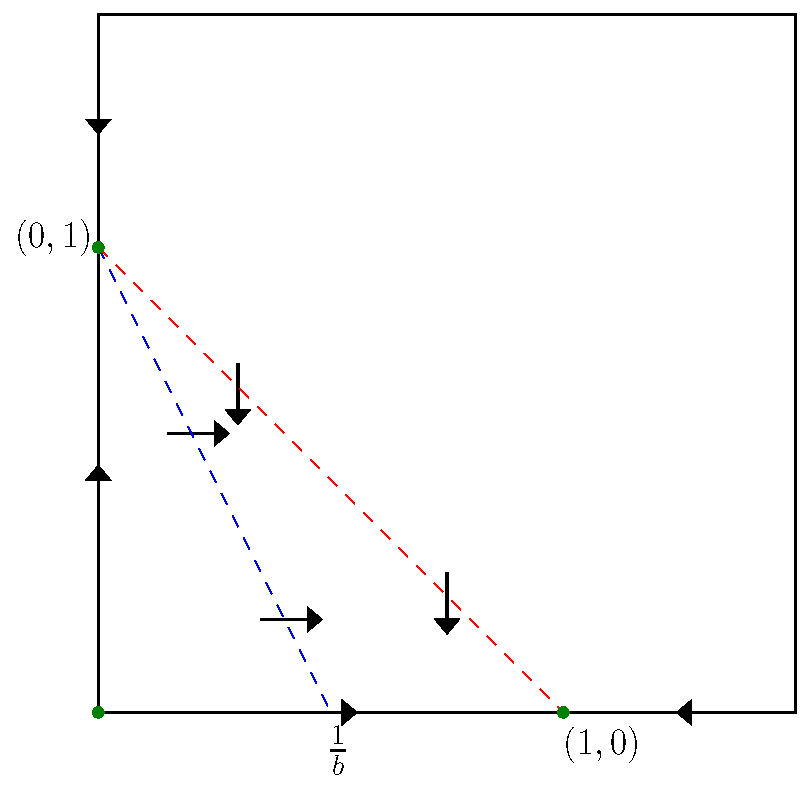
\includegraphics[width=\textwidth]{retrat-5a.pdf}
		\caption{Regions invariants del pla i nulclines}
		\label{fig:retrat 5a}
	\end{subfigure}
	\begin{subfigure}[htb]{0.48\textwidth}
		\centering
		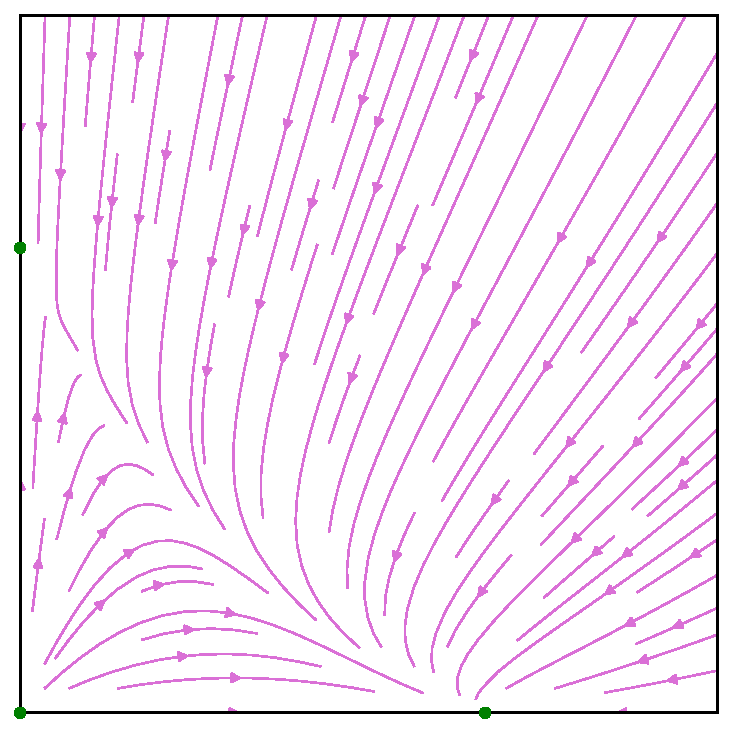
\includegraphics[width=\textwidth]{retrat-5b.pdf}
		\caption{Retrat de fase}
		\label{fig:retrat 5b}
	\end{subfigure}
	\caption{Anàlisi del sistema en el cas \( a = 1 \), \( b > 1 \)}
	\label{fig:retrat 5}
\end{figure}

Quan \( a = 1 \) i \( b > 1 \) la situació és diferent. Ara \( (1,0) \) es manté hiperbòlic però passa a ser una sella. No tenim prou informació per a saber si les òrbites que entren dins de la regió positivament invariant delimitada per les nulclines moren a \( (1,0) \) o a \( (0,1) \). Ara bé, com que en aquesta zona la component horitzontal del camp és sempre positiva i la component vertical és sempre negativa, podem intuir que les òrbites de fet tenen \( \omega \)-límit \( (1,0) \). Pel que fa a l'\( \alpha \)-límit, en qualsevol entorn de l'origen que només el tingui a ell com a punt crític, les òrbites han de tenir \( \alpha \)-límit l'origen, per Poincaré-Bendixson, de manera que les òrbites per sota de la nulclina inferior no poden tenir \( \alpha \)-límit \( (0,1) \). A la \cref{fig:retrat 5b} es mostra el retrat de fase del sistema calculat numèricament, el qual deixa intuir que \( (0,1) \) de fet és una sella.

\parbreak 

Si interpretem el model en termes de població, veiem que és un model que té en compte una taxa de creixement fixa per a ambdues poblacions, així com competència tant intraespecífica com interespecífica. Aquesta última és la que governen els paràmetres \( a \) i \( b \). Quan \( a,b < 1 \) la competència interespecífica és prou petita i les poblacions poden conviure, ja que tota condició inicial tendeix cap al valor estable \( P \). 

En canvi, si \( a, b > 1 \) la competència és massa gran i només sobreviu una de les espècies, ja que tota condició inicial tendeix cap a \( (1,0) \), és a dir, l'extinció de l'espècie \( y \) o \( (0,1) \), l'extinció de l'espècie \( y \). Quina de les dues espècies s'extingeix ve determinat per l'òrbita heteroclínica que va de l'origen fins a \( P \), i que actua com a separatriu. Existeix la possibilitat de coexistència ja que tenim un punt de sella, però és molt fràgil. 

Si \( a \geq 1 \) i \( b < 1 \) aleshores l'espècie \( y \) és molt competitiva i l'espècie \( x \) és poc competitiva, de manera que s'acaba extingint, ja que tota trajectòria acaba tendint a \( (0,1) \), és a dir, a l'extinció de \( x \). Finalment, si	\( a = 1 \) i \( b > a \) aleshores s'extingirà l'espècie \( y \). En aquests dos últims casos no hi ha possibilitat de coexistència. 

\parbreak

\begin{figure}
	\centering
	\begin{subfigure}[htb]{0.48\textwidth}
		\centering
		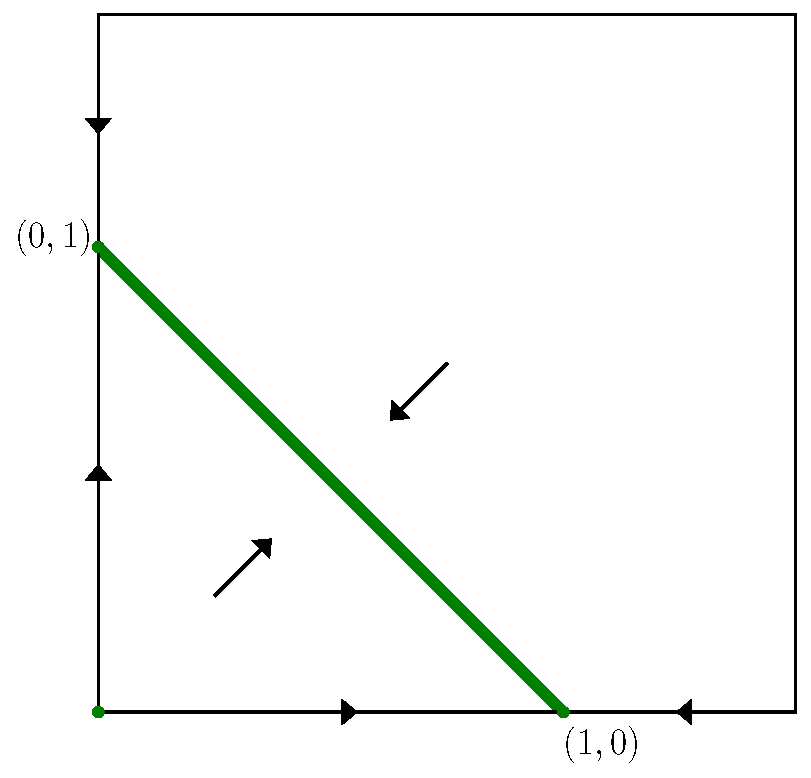
\includegraphics[width=\textwidth]{retrat-6a.pdf}
		\caption{Regions invariants del pla i nulclines}
		\label{fig:retrat 6a}
	\end{subfigure}
	\begin{subfigure}[htb]{0.48\textwidth}
		\centering
		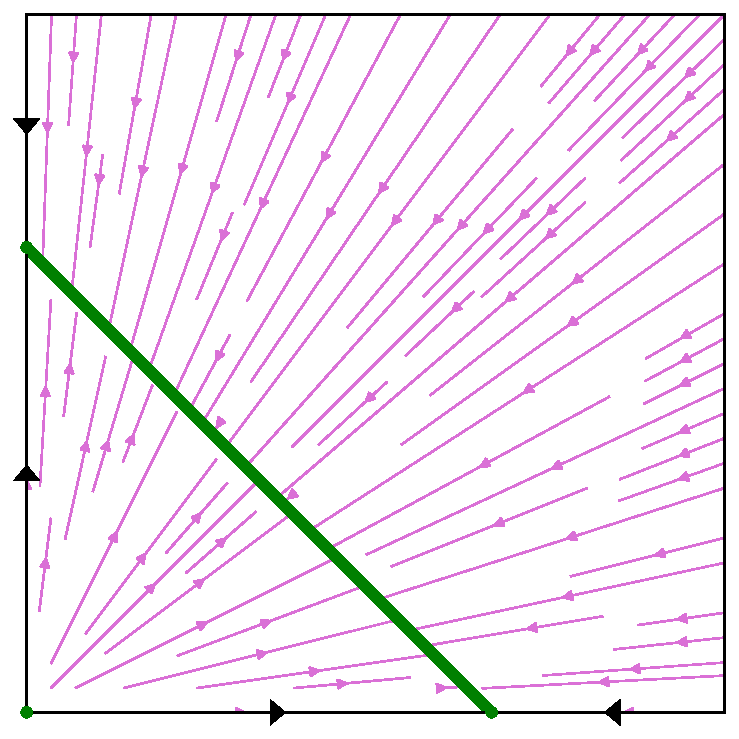
\includegraphics[width=\textwidth]{retrat-6b.pdf}
		\caption{Retrat de fase}
		\label{fig:retrat 6b}
	\end{subfigure}
	\caption{Anàlisi del sistema en el cas \( a = 1 \), \( b > 1 \)}
	\label{fig:retrat 6}
\end{figure}

Quan \( a = b = 1 \) aleshores la recta \( x + y = 1 \) esdevè una recta de punts fixos. Com que són aïllats ja no són hiperbòlics i no podem aplicar-hi Hartman per conèixer-ne la dinàmica local. Podem afirmar que el sistema no pot tenir òrbites periòdiques que no tallin la recta de punts crítics, ja que si fos així haurien d'envoltar algun punt crític fora de la recta de punts crítics, que no existeix. Tampoc podrien existir òrbites periòdiques que sí que talléssin la recta de punts crítics ja uqe en general les òrbites no es poden tallar. Per a determinar la dinàmica en general del sistema observem que 
\begin{equation*}
	x\dot{y} - y\dot{x} = xy(1 - x - y) - yx(1 - x - y) = 0
\end{equation*}
i per tant \( \dot{\theta} = 0 \). En particular tenim que totes les rectes que passen per l'origen són invariants. Si calculem els signes dels components del camp trobem el que es veu a la \cref{fig:retrat 6a}. Amb això ja tenim determinada la dinàmica: si un punt comença per sobre de la recta \( x + y = 1 \) aleshores es mou al llarg de la recta que l'uneix amb l'origen fins a la recta de punts fixos. I si comença per sota també es veu atret. Així l'\( \omega \)-límit de qualsevol punt no fix és la intersecció de la recta que l'uneix amb l'origen i la recta \( x+y = 1 \).  

Pel que fa a la dinàmica de poblacions, el que passa és que si la població total \( x + y \) és més gran que 1, aleshores la població d'ambdues espècies decreix mantenint la proporció entre les poblacions constant fins a estabilitzar-se a una població total de 1. I si \( x+y < 1 \) l'evolució és la mateixa però la població total creix cap a 1. 

\addtocounter{section}{2}
\addtocounter{section}{-1}
\setcounter{equation}{0}
\section*{Problema 2}
Hem d'analitzar la dinàmica del sistema de Liénard
\begin{equation} \label{eqn:sistema lienard}
	\left\{
		\begin{aligned}
			\dot{x} &= y - F(x) \\
			\dot{y} &= -x.
		\end{aligned}
	\right.
\end{equation}
Concretament hem de donar condicions sobre \( F \) de manera que el sistema tingui com a màxim una o cap òrbita periòdica. L'eina idònia per aquesta mena de càlculs és el teorema de Bendixson-Dulac. Seguint la indicació, es proposa de trobar una funció de Dulac de la forma
\begin{equation*}
    B(x,y) = \frac{1}{y^2 + a(x)y + b(x)}
\end{equation*}
de manera que el numerador de \( \div{(B(x,y)X(x,y))} \) només depengui de \( x \), sent \( X \) el camp associat al sistema de Liénard. Si fem el càlcul obtenim
\begin{align*}
    \div{(B(x,y)X(x,y))} &= \frac{-(F'(x) + a'(x))y^2 + (a'(x)F(x) - a(x)F'(x) - b'(x) + 2x)y }{(y^2 + a(x)y + b(x))^2} \\
    &+ \frac{- F'(x)b(x) + F(x)b'(x) + xa(x)}{(y^2 + a(x)y + b(x))^2}.
\end{align*}
Si volem que el numerador només depengui de \( x \) podem posar \( a(x) = -F(x) \). Aleshores el terme amb \( y \) es converteix en \( -b'(x) + 2x \). Si volem anu\l.lar-lo podem triar \( b(x) = x^2 \). Amb aquesta tria la funció de Dulac esdevé
\begin{equation*}
    B(x,y) = \frac{1}{y^2 - F(x)y + x^2}
\end{equation*}
i la divergència
\begin{equation*}
    \div{(B(x,y)X(x,y))} = \frac{xF(x) - x^2 F'(x)}{(y^2 - F(x)y + x^2)^2}.
\end{equation*}
Per a poder aplicar el teorema de Bendixson-Dulac necessitem que \( B \) estigui definida sobre una regió \( U \) i que \( \div{(BX)} \) no canviï de signe sobre \( U \), tret de sobre conjunts de mesura 0. En aquestes condicions, si \( U \) és simplement connex aleshores podem afirmar que el sistema no té òrbites periòdiques completament contingudes dins de \( U \). I si \( U \) té un forat aleshores el sistema pot tenir com a molt una òrbita periòdica que envolta el forat.

Tenim que la funció de Dulac \( B \) està definida a tot arreu on el seu denominador no s'anu\l.li. Serà efectivament de Dulac si \( xF(x) - x^2F'(x) \) no canvia de signe sobre el domini de definició. Per tant ens interessa saber com és el conjunt
\begin{equation*}
    S = \{(x,y) \in \R^2 \mid y^2 - F(x)y + x^2 = 0 \}.
\end{equation*}
Sigui quina sigui \( F \), el punt \( (0,0) \) és de \( S \). Si aconseguim donar condicions de manera que \( S \) sigui un punt estarem en situació per aplicar Bendixson-Dulac, ja que tindrem una funció de Dulac definida sobre un conjunt amb un forat, i per tant podrem tenir com a molt una òrbita periòdica. Ara bé, si el punt en qüestió no és crític sabem que no hi haurà possibilitat de tenir cap òrbita periòdica. Com que l'únic punt crític del sistema de Liénard és \( (0, F(0)) \) és raonable requerir \( F(0) = 0 \) de manera que el punt en el qual la funció de Dulac no està definida coincideix amb el punt crític del sistema i per tant hi ha esperança de tenir una òrbita periòdica. 

Volem, doncs, aconseguir que \( S \) estigui buit a part de \( (0,0) \). Això ho aconseguim imposant que el discriminant \( F(x)^2 - 4x^2 \) sigui negatiu, de manera que el conjunt de solucions de \( y^2 - F(x)y + x^2 = 0 \) sigui buit, tret de \( (0,0) \) quan \( x = 0 \). 

En resum, si \( F \) satisfà
\begin{itemize}
    \item \( xF(x) - x^2F'(x) \) no canvia de signe sobre \( \R^2 - {(0,0)} \),
    \item \( F(0) = 0 \),
    \item i \( F(x)^2 < 4x^2 \) per \( \abs{x} > 0 \)
\end{itemize}
aleshores el sistema de Liènard corresponent pot tenir com a molt una òrbita periòdica que envolta l'origen.

Pel que fa al cas en el que el sistema no tingui òrbites periòdiques, una bona font d'exemples és quan \( F \) és lineal. Posem \( F(x) = ax \), de manera que el sistema esdevé
\begin{equation*}
    \left\{
		\begin{aligned}
			\dot{x} &= y - ax \\
			\dot{y} &= -x.
		\end{aligned}
	\right.
\end{equation*}
El sistema té valors propis
\begin{equation*}
    \lambda_1 = \frac{-a + \sqrt{a^2 - 4}}{2}
\end{equation*}
i 
\begin{equation*}
    \lambda_2 = \frac{-a - \sqrt{a^2 - 4}}{2}.
\end{equation*}
Només podrà tenir òrbites periòdiques si és un centre, i només serà un centre si la part real dels valors propis és 0. Per tant, si \( a \neq \) podem garantir que el sistema no tindrà òrbites periòdiques.

\parbreak

Considerem \( F(x) = \frac{x(1 - cx^2)}{1 + cx^2} \) amb \( c > 0 \) i comprovem si verifica les condicions de l'apartat anterior per a la possibilitat de tenit com a molt un cicle límit. És clar que \( F(0) = 0 \). També tenim 
\begin{align*}
    F(x)^2 - 4x^2 & = \frac{x^2(1 - cx^2)^2}{(1 + cx^2)^2} - \frac{4x^2(1 + cx^2)^2}{(1 + cx^2)^2} \\
    & = -\frac{3x^2 + 10cx^2 - 3c^2x^6}{(1 + cx^2)^2} < 0
\end{align*}
si \( x \neq 0 \). 

Finalment
\begin{equation*}
    xF(x) = \frac{x^2(1 - cx^2)(1 + cx^2)}{(1 + cx)^2} = \frac{x^2 - c^2x^6}{(1 + cx^2)^2}
\end{equation*}
i
\begin{equation*}
    F'(x) = \frac{1 - 4cx^2 - c^2x^4}{(1 + cx^2)^2}
\end{equation*}
per tant
\begin{equation*}
    xF(x) - x^2F'(x) = \frac{4cx^2}{(1 + cx^2)^2} > 0
\end{equation*}
si \( \abs{x} > 0 \). Així doncs estem en les hipòtesis de l'apartat anterior i podem afirmar, per Bendixson-Dulac, que el sistema té com a màxim una òrbita periòdica.
\end{document}

